\documentclass[aspectratio=169, table]{beamer}

\usepackage[utf8]{inputenc}
\usepackage{listings} 

\usetheme{Pradita}

\subtitle{MTI104 - IT Services}

\title{Session-02:\\\LARGE{ITIL 101: Concepts and\\Core Foundation}}
\date[Serial]{\scriptsize {PRU/SPMI/FR-BM-18/0222}}
\author[Pradita]{\small{\textbf{Alfa Yohannis}}}

\begin{document}

\frame{\titlepage}

\begin{frame}{Introduction}
	\begin{itemize} 
		\item ITIL 4 Foundation Certification exam study guide starts with this chapter.
		\item Chapter 1: Nuances and history of ITIL.
		\item Chapter 2: Insight into the world of DevOps and its practices.
		\item This chapter focuses on ITIL concepts and service management.
		\item Topics include value, outcomes, costs, and risks.
		\item Discussion on service relationships.
		\item Exam tips and typical questions.
	\end{itemize}
\end{frame}

\begin{frame}{Service Provider and Consumer}
\begin{center}
	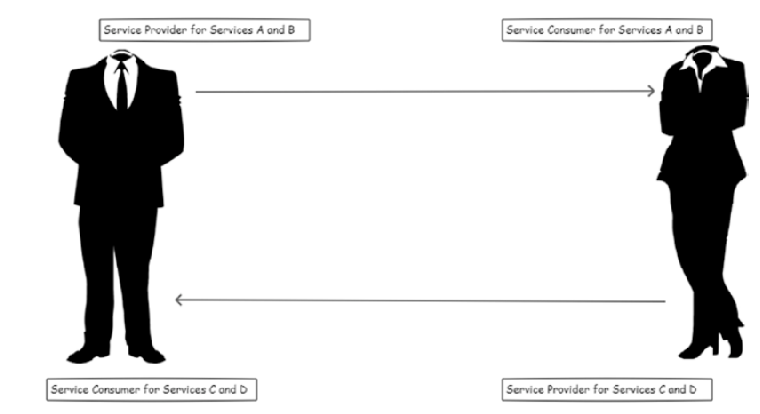
\includegraphics[width=0.8\linewidth]{images/image-01.png}
\end{center}
\end{frame}

\begin{frame}{Service Management}
	\begin{itemize}
		\item Importance of service-related options in products.
		\item Example: Apple and its service factor.
		\item A brand's value from services.
		\item Service provider's role in keeping things in motion.
		\item Tangibles (e.g., iPhone, Tesla) and intangibles (e.g., electricity).
		\item Services collectively fall under service management.
		\item Specializations: IT, hospitality, medicine.
	\end{itemize}
\end{frame}

\begin{frame}{ITIL Definition of Service Management}
	\begin{itemize}
		\item A set of specialized organizational capabilities for enabling value for customers in the form of services.
		\item Technical maturity, experience, customer service, and management frameworks.
		\item Leadership in service management.
		\item Reading stakeholders accurately.
		\item Service management as part of product management.
		\item Product and service synergy.
		\item Exam tip: Memorize definitions.
	\end{itemize}
\end{frame}

\begin{frame}{Products and Services}
	\begin{itemize}
		\item Closing gulf between products and services.
		\item Digital age trend: products as services.
		\item Example: MS Office to Office 365.
		\item ITIL's focus on services.
		\item ITIL Definition of a Product.
		\item Configuration of an organization's resources designed to offer value.
		\item Multiple forms of resources: people, processes, products.
	\end{itemize}
\end{frame}

\begin{frame}{ITIL Definition of a Service}
	\begin{itemize}
		\item A means of enabling value co-creation by facilitating outcomes customers want to achieve.
		\item Service provider owns risks and costs.
		\item Office 365 example: benefits and responsibilities.
		\item Continuous improvement and imagination.
		\item Active customer involvement.
		\item Service provider's competitive pricing.
		\item Exam tip: Understand the service definition.
	\end{itemize}
\end{frame}

\begin{frame}{Organization}
	\begin{itemize}
		\item Value creation with support and feedback.
		\item ITIL Definition of an Organization.
		\item Person or group with responsibilities, authorities, and relationships.
		\item Organizational roles: service provider and service consumer.
		\item Example: Microsoft and Verizon.
		\item Contextual roles in different services.
		\item Service provider and consumer mutual relationship.
	\end{itemize}
\end{frame}

\begin{frame}{People Roles}
	\begin{itemize}
		\item Generic roles: customer, sponsor, user.
		\item ITIL Definition of a Customer.
		\item Customer defines service requirements.
		\item ITIL Definition of a Sponsor.
		\item Sponsor authorizes budget for service consumption.
		\item ITIL Definition of a User.
		\item User enjoys and provides feedback on the service.
	\end{itemize}
\end{frame}

\begin{frame}{Examples and Exam Tips}
	\begin{itemize}
		\item Example: Multinational organization and laptops.
		\item Example: Mom and pop grocery shop.
		\item Customer, sponsor, and user roles.
		\item Exam tip: Expect 1-2 questions from this section.
	\end{itemize}
\end{frame}

\end{document}
